\documentclass[17pt]{extarticle} % another possible option: 20 pt
\usepackage{ifpdf}
\ifpdf
\usepackage{cmap}
\fi
\usepackage[english]{babel}
\usepackage{palatino}
\usepackage[x11names,svgnames]{xcolor}
\usepackage{amsmath,amssymb,amsfonts}
\usepackage{tikz}
\usepackage{amsthm}
\usepackage{pgf}
\usepackage{multicol}
\usepackage{xspace}
\usepackage{graphicx}
\usepackage{multicol}
\usepackage[section]{algorithm} % [section] is use to define the numbering mode
\usepackage{algorithmic} 
\usepackage[a1paper,left=2.5cm,right=.5cm,top=2.5cm,bottom=.5cm,foot=0cm]{geometry}
\usepackage{poster}
\usepackage{booktabs}
\usepackage{multirow,multicol}

\usetikzlibrary{positioning,fadings}

\usepackage{pgfplots}

\theoremstyle{definition}
\newtheorem{definition}{Definition}[section]
\newtheorem{proposition}{Proposition}[section]
\newtheorem{corollary}{Corollary}[section]
\newtheorem{theorem}{Theorem}[section]
                             

\def\nodeshadowed[#1]#2;{
\node[scale=2,above,#1]{#2};
\node[scale=2,above,#1,yscale=-1,opacity=0.4]{#2};}

\begin{document}
\pagestyle{empty}

%%% RAMKA
%\noindent\hspace{-2cm}
%\begin{tikzpicture}[rounded corners=2cm,x=1cm,y=1cm]
%  \draw (0,-1) [color=SteelBlue3,line width=2mm] rectangle (55.5,79);
%\end{tikzpicture}
%\vspace{-78.5cm}

%%% TITLE
%\begin{center}
  %{\color{OrangeRed} \fontsize{48pt}{1em} {\bf Earmark graph approach to {\it de novo} genome assembly}}
  %\vspace{1.5cm}
    
  %\fontsize{32pt}{2.5em}\selectfont
  %\color{DodgerBlue3}
  %{\bf Mikhail Dvorkin, Alexander S. Kulikov, Max Alekseyev}
  %{affiliations}
  %{\tt emails}
%\end{center}%
%\vspace{1cm}

%\fontsize{32pt}{2.5em}\selectfont

\begin{center}
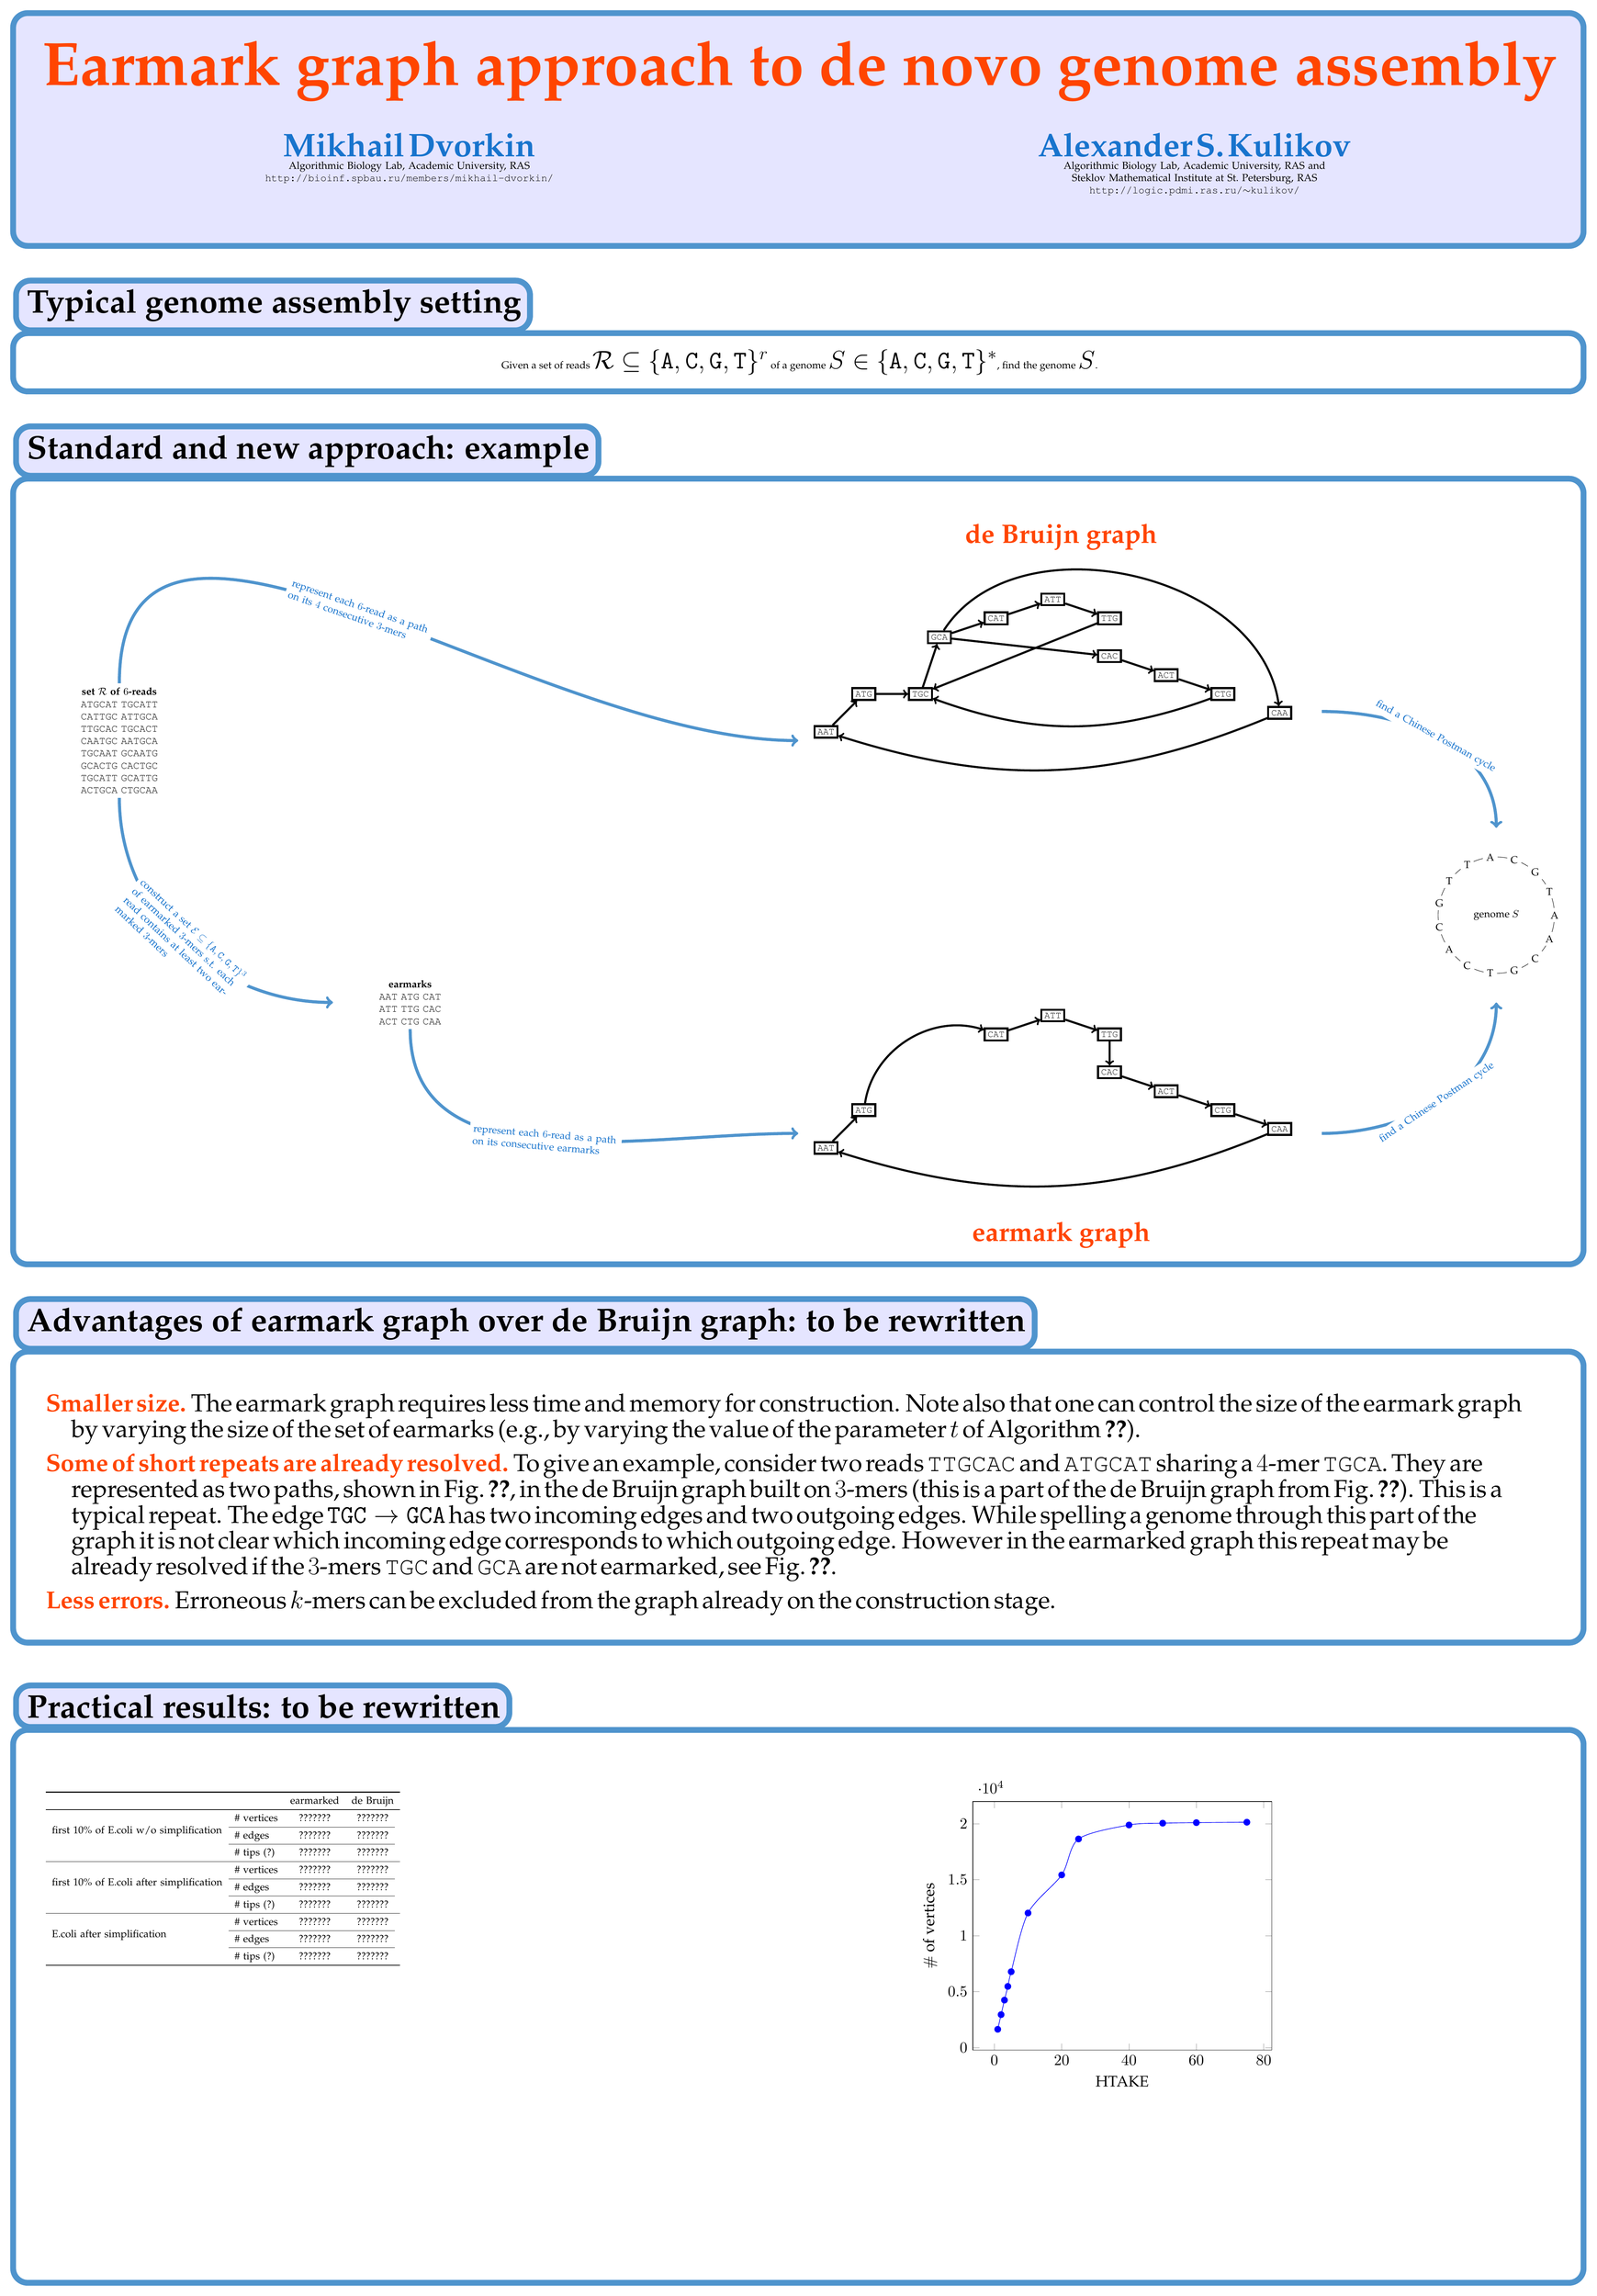
\begin{tikzpicture}

%%%%%%%%%%%%%%%GRID
%\draw[step=1cm,help lines] (0,0) grid (54,78);
%\foreach \x in {0,...,54} { \node at (\x,-1) {$\x$}; \node at (\x,79) {$\x$}; }
%\foreach \x in {0,...,78} { \node at (-1,\x) {$\x$}; \node at (55,\x) {$\x$}; }

%%%%%%%%%%%%%%%TITLE
\begin{scope}
\draw (0,78) [color=SteelBlue3,line width=2mm,rounded corners=.5cm,fill=blue!10!white] rectangle (54,70);
\node at (27,76) {\color{OrangeRed} \fontsize{60pt}{1em} \bf Earmark graph approach to de novo genome assembly};
\node[rectangle,text width=25cm,text centered,anchor=north west] at (1,74) {
  {\bf \color{DodgerBlue3} \fontsize{32pt}{1em}\selectfont Mikhail Dvorkin}\\
  Algorithmic Biology Lab, Academic University, RAS\\
  {\tt http://bioinf.spbau.ru/members/mikhail-dvorkin/}
};
\node[rectangle,text width=25cm,text centered,anchor=north west] at (28,74) {
  {\bf \color{DodgerBlue3} \fontsize{32pt}{1em}\selectfont Alexander S. Kulikov}\\
  Algorithmic Biology Lab, Academic University, RAS and\\
  Steklov Mathematical Institute at St.~Petersburg, RAS\\
  {\tt http://logic.pdmi.ras.ru/$\sim$kulikov/}
};

\end{scope}

%%%%%%%%%%%%%%%PROBLEM STATEMENT
\begin{scope}[yshift=-4cm]
\draw (0,71) [color=SteelBlue3,line width=2mm,rounded corners=.5cm] rectangle (54,69);
\node[draw=SteelBlue3,line width=2mm,rounded corners=.5cm,anchor=south west,fill=blue!10!white,inner sep=3mm] at (0,71) {\fontsize{32pt}{1em} 
\bf Typical genome assembly setting};
\node at (27,70) {\fontsize{26pt}{1em} Given a set of reads ${\cal R} \subseteq \{{\tt 
A,C,G,T}\}^r$ of a genome $S \in \{{\tt A,C,G,T}\}^*$, find the genome $S$.};
\end{scope}

%%%%%%%%%%%%%%%EXAMPLE
\begin{scope}%[yshift=-4cm]
  \draw (0,62) [color=SteelBlue3,line width=2mm,rounded corners=.5cm] rectangle (54,35);
  \node[draw=SteelBlue3,line width=2mm,rounded corners=.5cm,anchor=south west,fill=blue!10!white,inner sep=3mm] at (0,62) {\fontsize{32pt}{1em} \bf 
    Standard and new approach: example};

  %%% READS
  \node[rectangle,line width=2pt,text width=5cm,text centered,anchor=west] (reads) at (1,53) {
    {\bf set ${\cal R}$ of $6$-reads}\\
    {\tt ATGCAT} {\tt TGCATT}\\
    {\tt CATTGC} {\tt ATTGCA}\\
    {\tt TTGCAC} {\tt TGCACT}\\
    {\tt CAATGC} {\tt AATGCA}\\
    {\tt TGCAAT} {\tt GCAATG}\\
    {\tt GCACTG} {\tt CACTGC}\\
    {\tt TGCATT} {\tt GCATTG}\\
    {\tt ACTGCA} {\tt CTGCAA}\\
  };

  %\draw [->,line width=2pt] (reads) to[out=90,in=180] node[sloped,fill=white] {de Bruijn graph} (23,53);
  %\draw [->,line width=2pt] (reads) to[out=-90,in=180] node[sloped,fill=white] {earmark graph} (23,44);



  \begin{scope}[scale=1.3,transform shape,line width=2pt]
    \begin{scope}[xshift=20cm,yshift=40cm]
      \foreach \x/\y/\t in {1.5/1/AAT, 2.5/2/ATG, 4/2/TGC, 4.5/3.5/GCA, 6/4/CAT, 
                            7.5/4.5/ATT, 9/4/TTG, 9/3/CAC, 10.5/2.5/ACT, 12/2/CTG,
                            13.5/1.5/CAA}
      \node[draw,rectangle,scale=0.7] (\t) at (\x,\y) {{\tt \t}};

      \foreach \s/\t in {AAT/ATG, ATG/TGC, TGC/GCA, GCA/CAT, CAT/ATT, ATT/TTG, TTG/TGC, 
                         GCA/CAC, CAC/ACT, ACT/CTG}
        \draw [->] (\s) to (\t);
      \draw [->] (GCA) to[bend left=70] (CAA);
      \draw [->] (CAA) to[bend left=20] (AAT);
      \draw [->] (CTG) to[bend left=20] (TGC);
      %\path[->] (GCA) edge [out=90,in=90] (CAA);
    \end{scope}

    \begin{scope}[xshift=20cm,yshift=29cm]
      \foreach \x/\y/\t in {1.5/1/AAT, 2.5/2/ATG, 6/4/CAT, 
                            7.5/4.5/ATT, 9/4/TTG, 9/3/CAC, 10.5/2.5/ACT, 12/2/CTG,
                            13.5/1.5/CAA}
      \node[draw,rectangle,scale=0.7] (\t) at (\x,\y) {{\tt \t}};

      \foreach \s/\t in {AAT/ATG, CAT/ATT, ATT/TTG, TTG/CAC, 
        CAC/ACT, ACT/CTG, CTG/CAA}
        \draw [->] (\s) to (\t);
      \draw [->] (CAA) to[bend left=20] (AAT);
      \draw [->] (ATG) to[bend left=50] (CAT);
    \end{scope}
  \end{scope}

  %\node at (47,59) {\includegraphics[width=7cm]{fu.jpg}};
  %\node at (45,44) {\includegraphics[width=7cm]{troll.jpg}};

  \begin{scope}[xshift=51cm,yshift=47cm]
    \draw (0,0) circle (2cm);
    \foreach \i/\a in {0/A,1/T,2/G,3/C,4/A,5/T,6/T,7/G,8/C,9/A,10/C,11/T,12/G,13/C,14/A} {
      \node[fill=white] at (360*\i/15:2cm) {\a};
    }
    \node at (0,0) {genome $S$};
  \end{scope}

  \node[rectangle,line width=2pt,text width=5cm,text centered,anchor=west] (earmarks) at (11,44) {
    {\bf earmarks}\\
    {\tt AAT} {\tt ATG} {\tt CAT}\\
    {\tt ATT} {\tt TTG} {\tt CAC}\\
    {\tt ACT} {\tt CTG} {\tt CAA}\\
  };


  \begin{scope}[draw=SteelBlue3,line width=3pt,fill=white]
    \draw [->] (reads) to[out=90,in=180] node[fill=white,sloped,rectangle,text width=5cm] 
      {\color{DodgerBlue3} represent each $6$-read as a path on its $4$ consecutive $3$-mers} (27,53);

    \draw [->] (45,54) to[out=0,in=90] node[fill=white,sloped,rectangle,text width=5cm] 
      {\color{DodgerBlue3} find a Chinese Postman cycle} (51,50);

    \draw [->] (45,39.5) to[out=0,in=-90] node[fill=white,sloped,rectangle,text width=5cm] 
      {\color{DodgerBlue3} find a Chinese Postman cycle} (51,44);

    \draw [->] (reads) to[out=-90,in=180] node[fill=white,sloped,rectangle,text width=5cm] 
      {\color{DodgerBlue3} construct a set ${\cal E} \subseteq \{{\tt A,C,G,T}\}^3$ of earmarked $3$-mers s.t. each read contains at least
      two earmarked $3$-mers} (earmarks);

    \draw [->] (earmarks) to[out=-90,in=180] node[fill=white,sloped,rectangle,text width=5cm] 
      {\color{DodgerBlue3} represent each $6$-read as a path on its consecutive earmarks} (27,39.5);
  \end{scope}

  \node at (36,60) {\fontsize{26pt}{1em} \color{OrangeRed} \bf de Bruijn graph};
  \node at (36,36) {\fontsize{26pt}{1em} \color{OrangeRed} \bf earmark graph};
\end{scope}

%%%%%%%%%%%%%%%ADVANTAGES
\begin{scope}%[yshift=-4cm]
  \draw (0,32) [color=SteelBlue3,line width=2mm,rounded corners=.5cm] rectangle (54,22);
  \node[draw=SteelBlue3,line width=2mm,rounded corners=.5cm,anchor=south west,fill=blue!10!white,inner sep=3mm] at (0,32) {\fontsize{32pt}{1em} \bf 
    Advantages of earmark graph over de Bruijn graph: to be rewritten};
  \node[rectangle,text width=51cm,anchor=north west] at (1,31) {
    \fontsize{24pt}{1em}\selectfont
    \begin{description}
    \item[\color{OrangeRed} \bf Smaller size.]
    The earmark graph requires less time and memory for construction.
    Note also that one can control the size of the earmark graph 
    by varying the size of the set of earmarks (e.g., by varying the value of the parameter $t$
    of Algorithm~\ref{alg:earmarksselection}).
    \item[\color{OrangeRed} \bf Some of short repeats are already resolved.]
    To give an example, consider two reads {\tt TTGCAC} and {\tt ATGCAT} 
    sharing a $4$-mer {\tt TGCA}. They are represented as two paths, shown 
    in Fig.~\ref{fig:repa}, in the de Bruijn graph built on $3$-mers
    (this is a part of the de Bruijn graph from Fig.~\ref{fig:debruijn}).
    This is a typical repeat. The edge ${\tt TGC}\rightarrow{\tt GCA}$ has two
    incoming edges and two outgoing edges. While spelling a genome
    through this part of the graph it is not clear which incoming edge 
    corresponds to which outgoing edge. However in the earmarked graph
    this repeat may be already resolved if the $3$-mers {\tt TGC} and {\tt GCA}
    are not earmarked, see Fig.~\ref{fig:repb}.
    \item[\color{OrangeRed} \bf Less errors.] Erroneous $k$-mers can be excluded from the graph already on
    the construction stage.
    \end{description}
  };
\end{scope}

%%%%%%%%%%%%%%%PRACTICAL RESULTS
\begin{scope}%[yshift=-4cm]
  \draw (0,19) [color=SteelBlue3,line width=2mm,rounded corners=.5cm] rectangle (54,0);
  \node[draw=SteelBlue3,line width=2mm,rounded corners=.5cm,anchor=south west,fill=blue!10!white,inner sep=3mm] at (0,19) {\fontsize{32pt}{1em} \bf 
    Practical results: to be rewritten};
  
  \begin{scope}[xshift=33cm,yshift=8cm,scale=1.5]
    \begin{axis}[xlabel={HTAKE},ylabel={$\#$ of vertices}]
    \addplot[smooth,mark=*,blue] plot coordinates { (1,1640) (2,2950) (3,4248) (4,5472) (5,6784)
      (10, 12028) (20, 15432) (25, 18642) (40, 19890) (50, 20052) (60, 20102) (75,20140) };
    %\addlegendentry{de Bruijn}
    \end{axis}
  \end{scope}

  \node[rectangle,text width=27cm,anchor=north west] at (1,17) {
    \begin{tabular}{llcc}
    \toprule
    & & earmarked & de Bruijn\\

    \midrule
    \multirow{3}{*}{first 10\% of E.coli w/o simplification} & \# vertices & ??????? & ???????\\
    \cmidrule(r){2-4}
    & \# edges & ??????? & ???????\\
    \cmidrule(r){2-4}
    & \# tips (?) & ??????? & ???????\\

    \midrule
    \multirow{3}{*}{first 10\% of E.coli after simplification} & \# vertices & ??????? & ???????\\
    \cmidrule(r){2-4}
    & \# edges & ??????? & ???????\\
    \cmidrule(r){2-4}
    & \# tips (?) & ??????? & ???????\\

    \midrule
    \multirow{3}{*}{E.coli after simplification} & \# vertices & ??????? & ???????\\
    \cmidrule(r){2-4}
    & \# edges & ??????? & ???????\\
    \cmidrule(r){2-4}
    & \# tips (?) & ??????? & ???????\\

    \bottomrule
    \end{tabular}
  };
\end{scope}


\end{tikzpicture}
\end{center}


\end{document}
